\documentclass[presentation]{beamer}
\mode<presentation>{\usetheme{AMSBolognaFCrev}}

\usepackage[utf8]{inputenc}
\usepackage[T1]{fontenc}
\usepackage{booktabs}
\usepackage{array}
\usepackage{colortbl}
\usepackage{tikz}
\usepackage[ddmmyyyy]{datetime}
\usepackage[export]{adjustbox}
\usetikzlibrary{arrows.meta,positioning,shapes.geometric}

\renewcommand{\dateseparator}{/}
\newcommand{\sectiontitleframe}[1]{
\begin{frame}[plain,c]
\begin{center}
{\usebeamerfont{title}\usebeamercolor[fg]{title}#1}
\end{center}
\end{frame}
}

\title[Lesson 4]{RBAC and Logging in OpenHospital}
\institute[Data Privacy and Security]{Healthcare Data Privacy and Security}
\author[\sspeaker{G. Pisano}]{\speaker{Giuseppe Pisano} \\\href{mailto:g.pisano@unibo.it}{g.pisano@unibo.it}}
\date[August, 2026]{August, 2026}
%
\titlegraphic{
\begin{center}
    
\includegraphics[width=0.35\textwidth, valign=c]{logos/intestazione.png}
    
\includegraphics[width=0.16\textwidth, valign=c]{logos/unibo_logo_2.png}
    
\includegraphics[width=0.11\textwidth, valign=c]{logos/makeni_logo_2.png}
    
\includegraphics[width=0.20\textwidth, valign=c]{logos/cuamm_logo_png.png}
\end{center}
\centering
\tiny{S.K.I.L.L.E.D --- AID013244/04/2\\Strategic Knowledge and Inclusive Lifelong Learning in the health sector for youth Employability and Development}
}

\begin{document}

\setbeamertemplate{frametitle}
{
    \nointerlineskip
    \begin{beamercolorbox}[sep=0.3cm,ht=2.2em,wd=\paperwidth]{frametitle}
        \vbox{}\vskip-2ex%
        \strut\insertframetitle\hfill\raisebox{-0.2\height}{
\includegraphics[width=2cm]{logos/cuamm_logo_png.png}}\strut
        \vskip-0.8ex%
    \end{beamercolorbox}
}

\begin{frame}[allowframebreaks]
\titlepage
\end{frame}

\begin{frame}[c,allowframebreaks]{Roadmap}
\tableofcontents[hideallsubsections]
\end{frame}

\begin{frame}[c]{Lab Goal}
\begin{block}{What we will do}
We will install a test OpenHospital instance, enable multi-user login, configure groups and users,
test which functions each group can access, and inspect what the application logs actually record.
\end{block}

\begin{exampleblock}{Why OpenHospital}
OpenHospital is a real healthcare application. Its access-control model is \textbf{RBAC-like}:
users belong to groups, and groups receive menu/function permissions from an administrator.
\end{exampleblock}
\end{frame}

\begin{frame}[c]{How This Lab Progresses}
\begin{block}{Learning path}
We move from \textbf{installation}, to \textbf{first run}, to \textbf{multi-user mode}, then to
\textbf{group policy}, \textbf{user accounts}, \textbf{access testing}, and finally to
\textbf{logging and audit-gap discussion}.
\end{block}

\begin{exampleblock}{Hospital storyline}
St. Isidore Hospital is piloting OpenHospital. The IT team must create distinct accounts for
registration staff, cashiers, clinicians, laboratory staff, pharmacy staff, and auditors.
\end{exampleblock}
\end{frame}

\begin{frame}[c]{Lab Safety}
\begin{block}{Important}
Use only a local test installation with demo or artificial data. Do not use real patient data,
personal staff credentials, or production systems during this lab.
\end{block}

\begin{exampleblock}{Operational rule}
If something goes wrong, delete the test folder or database and start again. The purpose is to learn
policy configuration, not to preserve a production deployment.
\end{exampleblock}
\end{frame}

\section{Preparation}
\sectiontitleframe{Preparation}

\begin{frame}[c]{Section Context: Preparation}
\begin{block}{What we are talking about}
Before touching access control, we need a working OpenHospital environment. The simplest option for
this lab is the portable/test setup because it avoids a full client/server deployment.
\end{block}
\end{frame}

\begin{frame}[c]{What OpenHospital Is}
\begin{block}{System profile}
OpenHospital is a free and open-source hospital information system developed in Java. It supports
standalone portable use and client/server configurations with a central database
\cite{openhospital_admin}.
\end{block}

\begin{exampleblock}{Healthcare relevance}
Its modules include patient registration, pharmacy, laboratory, outpatient management, admissions,
billing, and statistics. That gives us realistic functions for access-control testing.
\end{exampleblock}
\end{frame}

\begin{frame}[c]{Recommended Lab Setup}
\begin{block}{Use portable mode first}
Use \textbf{portable mode} or a single-machine test setup. It is easier to reset and it keeps the
focus on users, groups, permissions, and logs.
\end{block}

\begin{exampleblock}{Why not start with client/server}
Client/server mode is valuable later, but it adds database networking, host firewalls, and client
configuration before the access-control workflow is clear.
\end{exampleblock}
\end{frame}

\begin{frame}[c]{Prerequisites}
\begin{block}{Before starting}
\begin{itemize}
    \item Download the latest OpenHospital release for your operating system.
    \item Unpack the archive into a writable folder.
    \item Check that the package includes its bundled JRE and portable MariaDB/MySQL server.
    \item Keep one untouched copy so the lab can be reset quickly.
\end{itemize}
\end{block}

\begin{exampleblock}{Source}
The OpenHospital administrator guide describes download, unpacking, installation modes, and Java
requirements \cite{openhospital_admin}.
\end{exampleblock}
\end{frame}

\begin{frame}[c]{Java Runtime}
\begin{block}{Default case}
The portable OpenHospital package normally includes its own Java Runtime Environment, so Java should
not need a separate installation for the lab.
\end{block}

\begin{exampleblock}{If Java is missing}
If the startup script reports that Java cannot be found, install a supported Java runtime for the
OpenHospital release, or configure the script variable \texttt{JAVA\_BIN} to point to a system Java
executable.
\end{exampleblock}
\end{frame}

\begin{frame}[c]{Folder Discipline}
\begin{block}{Practical habit}
Create a dedicated lab folder such as \texttt{OpenHospital-Lab}. Avoid spaces and unusual
characters in the path if possible. Make sure the user running OpenHospital has read/write
permission on the extracted folder.
\end{block}

\begin{exampleblock}{Hospital example}
St. Isidore IT keeps the pilot under a clearly named test directory, separate from real hospital
systems and backups.
\end{exampleblock}
\end{frame}

\begin{frame}[c]{Checkpoint: Preparation}
\begin{block}{You are ready when}
\begin{itemize}
    \item OpenHospital is downloaded.
    \item The package is fully unpacked.
    \item The folder is writable.
    \item You know how to start the application on your operating system.
\end{itemize}
\end{block}
\end{frame}

\section{First Run}
\sectiontitleframe{First Run}

\begin{frame}[c]{Section Context: First Run}
\begin{block}{What we are talking about}
The first run confirms that the application works before we modify security settings. This creates a
known-good baseline.
\end{block}

\begin{exampleblock}{Practical rule}
Do not begin by editing configuration files. First prove that the application starts in its default
state.
\end{exampleblock}
\end{frame}

\begin{frame}[c]{Start OpenHospital}
\begin{block}{Action}
Run the provided OpenHospital startup script for your operating system from the extracted folder.
Use the official startup script rather than double-clicking random internal files.
\end{block}

\begin{exampleblock}{Expected observation}
On Linux, run \texttt{./oh.sh}. On Windows, run \texttt{oh.bat}; it launches \texttt{oh.ps1} and
shows the interactive menu. OpenHospital should then show its startup window or login window.
\end{exampleblock}
\end{frame}

\begin{frame}[c]{Startup Menu}
\begin{block}{Useful options}
The portable startup menu can select \textbf{PORTABLE}, \textbf{CLIENT}, or \textbf{SERVER} mode,
change language, toggle debug logging, initialize demo data, test database settings, and reset the
installation.
\end{block}

\begin{exampleblock}{Lab choice}
Use \textbf{PORTABLE} mode for this lab. Demo data can be useful for exploration, but enabling it
may require deleting/resetting portable data.
\end{exampleblock}
\end{frame}

\begin{frame}[c]{Windows Startup Notes}
\begin{block}{If Windows blocks the script}
The Windows launcher \texttt{oh.bat} starts \texttt{oh.ps1}. If PowerShell blocks it, open the file
properties for \texttt{oh.ps1}, choose \textbf{Unblock}, then run it again.
\end{block}

\begin{exampleblock}{Command-line fallback}
From PowerShell, the README shows this form:
\texttt{powershell.exe -ExecutionPolicy Bypass -File ./oh.ps1}.
\end{exampleblock}
\end{frame}

\begin{frame}[c]{Debug and Reset Options}
\begin{block}{Useful during the lab}
The startup menu can toggle \textbf{DEBUG} logging, generate configuration files, initialize demo
data, export or restore the database, and clean/reset the portable installation.
\end{block}

\begin{exampleblock}{Warning}
Use reset and demo initialization carefully: they may delete or overwrite portable data. This is
acceptable only when working on a disposable lab copy.
\end{exampleblock}
\end{frame}

\begin{frame}[c]{Checkpoint: First Run}
\begin{block}{Record your baseline}
\begin{itemize}
    \item Did the application start?
    \item Did it ask for a login?
    \item Which menu areas are visible?
    \item Where is the configuration folder?
    \item Where are logs written?
\end{itemize}
\end{block}
\end{frame}

\section{Confirm Login Mode}
\sectiontitleframe{Confirm Login Mode}

\begin{frame}[c]{Section Context: Login Mode}
\begin{block}{What we are talking about}
To study RBAC-like behavior, OpenHospital must ask users to log in. In the portable package this
may already be configured, so first observe the actual startup behavior.
\end{block}

\begin{exampleblock}{Hospital lens}
St. Isidore cannot manage accountability if all staff effectively act as the same user. Multi-user
mode is the doorway to meaningful authorization and audit.
\end{exampleblock}
\end{frame}

\begin{frame}[c]{If Login Already Appears}
\begin{block}{Action}
If OpenHospital starts with a login window, continue directly with the administrator account:
\texttt{admin} / \texttt{admin}.
\end{block}

\begin{exampleblock}{Security discussion}
This is the expected behavior in many current portable packages. In a real deployment, default
credentials must be changed immediately.
\end{exampleblock}
\end{frame}

\begin{frame}[c]{If Login Does Not Appear}
\begin{block}{Action}
Use the startup script configuration. In the portable scripts, single/multi-user behavior is
controlled by \texttt{OH\_SINGLE\_USER} on Linux or
\texttt{\$script:OH\_SINGLE\_USER} on Windows.
\end{block}

\begin{exampleblock}{Expected setting}
For this lab, the value should be \texttt{no}. The README also shows that configuration files can be
generated from the startup scripts when needed.
\end{exampleblock}
\end{frame}

\begin{frame}[c]{Configuration Files}
\begin{block}{Where to look}
The portable scripts create and manage runtime folders such as \texttt{data/conf},
\texttt{data/db}, \texttt{data/log}, \texttt{data/photo}, and OpenHospital resource files under
\texttt{oh/rsc}.
\end{block}

\begin{exampleblock}{Practical warning}
Do not edit random files while OpenHospital is running. If you need to change startup behavior, stop
the app, adjust the startup script or generated configuration intentionally, then restart.
\end{exampleblock}
\end{frame}

\begin{frame}[c]{Default Portable Folders}
\begin{center}
\scriptsize
\renewcommand{\arraystretch}{1.2}
\begin{tabular}{>{\bfseries}p{0.28\textwidth} p{0.48\textwidth}}
\toprule
Folder & Purpose \\
\midrule
\texttt{oh} & OpenHospital application files \\
\texttt{sql} & Database creation scripts \\
\texttt{data/conf} & MariaDB/MySQL configuration \\
\texttt{data/db} & Portable database files \\
\texttt{data/log} & Startup and application logs \\
\texttt{data/photo} & Patient photo storage \\
\texttt{data/dump} & Database exports/backups \\
\bottomrule
\end{tabular}
\end{center}
\end{frame}

\begin{frame}[c]{Checkpoint: Login Mode}
\begin{block}{You have succeeded when}
\begin{itemize}
    \item OpenHospital shows a login prompt.
    \item The \texttt{admin} account can log in.
    \item The user/group management menu is reachable from Settings.
    \item You can explain why shared/default accounts are unsafe in production.
\end{itemize}
\end{block}
\end{frame}

\section{Design the RBAC Policy}
\sectiontitleframe{Design the RBAC Policy}

\begin{frame}[c]{Section Context: Policy Design}
\begin{block}{What we are talking about}
Before clicking permissions, we design the policy. The administrator should know which job functions
exist and which system functions each job needs.
\end{block}

\begin{exampleblock}{Hospital lens}
This is where system administration meets governance. The tool enforces settings, but the hospital
decides the policy.
\end{exampleblock}
\end{frame}

\begin{frame}[c]{OpenHospital Model}
\begin{block}{RBAC-like structure}
OpenHospital manages users organized into groups. Each group is characterized by administrator
assigned permissions \cite{openhospital_user}.
\end{block}

\begin{exampleblock}{Classification}
Treat OpenHospital as \textbf{application-level RBAC-like access control}: users
map to groups, and groups map to menu/function permissions.
\end{exampleblock}
\end{frame}

\begin{frame}[c]{Scheme: OpenHospital Access Model}
\begin{center}
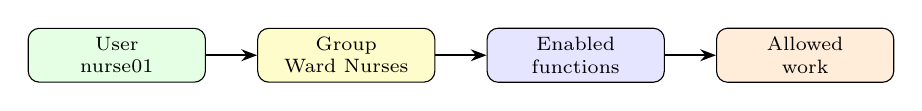
\begin{tikzpicture}[
    node distance=0.65cm,
    box/.style={draw, rounded corners, align=center, minimum width=2.25cm, minimum height=0.68cm, font=\scriptsize},
    link/.style={-{Stealth[length=2mm]}, thick}
]
\node[box, fill=green!10] (user) {User\\nurse01};
\node[box, right=of user, fill=yellow!20] (group) {Group\\Ward Nurses};
\node[box, right=of group, fill=blue!10] (menu) {Enabled\\functions};
\node[box, right=of menu, fill=orange!15] (action) {Allowed\\work};
\draw[link] (user) -- (group);
\draw[link] (group) -- (menu);
\draw[link] (menu) -- (action);
\end{tikzpicture}
\end{center}

\begin{block}{Reading the scheme}
Access is not delegated by file owners. It is centrally configured through group permissions.
\end{block}
\end{frame}

\begin{frame}[c]{Policy Scenario}
\begin{block}{Groups to create}
\begin{itemize}
    \item \textbf{Registration}: register and search patients.
    \item \textbf{Cashiers}: manage patient bills and payments.
    \item \textbf{Laboratory}: manage lab exams and results.
    \item \textbf{Pharmacy}: manage medicines and stock.
    \item \textbf{Auditors}: review data but avoid operational changes where possible.
\end{itemize}
\end{block}
\end{frame}

\begin{frame}[c]{Policy Matrix}
\begin{center}
\scriptsize
\renewcommand{\arraystretch}{1.15}
\begin{tabular}{@{}>{\bfseries}p{0.18\textwidth} p{0.15\textwidth} p{0.15\textwidth} p{0.15\textwidth} p{0.15\textwidth}@{}}
\toprule
Group & Patients & Billing & Lab & Pharmacy \\
\midrule
Registration & Create/search & No & No & No \\
Cashiers & Read only & Create/update & No & No \\
Laboratory & Read only & No & Create/update & No \\
Pharmacy & Read only & No & No & Create/update \\
Auditors & Review & Review & Review & Review \\
\bottomrule
\end{tabular}
\end{center}

\begin{block}{Practical note}
Exact menu names may differ. Map the policy intent to the nearest OpenHospital menu/function items.
\end{block}
\end{frame}

\begin{frame}[c]{Least Privilege Rule}
\begin{block}{Policy rule}
Start from what each group needs for routine work. Do not enable extra functions just because they
are convenient during setup.
\end{block}

\begin{exampleblock}{Hospital example}
Cashiers need billing functions. They do not need laboratory-result entry or pharmacy stock
management.
\end{exampleblock}
\end{frame}

\begin{frame}[c]{Checkpoint: Policy Design}
\begin{block}{Before configuration}
\begin{itemize}
    \item List each group.
    \item Write the work each group must perform.
    \item Write one action each group must \textbf{not} perform.
    \item Decide which tests will prove the policy works.
\end{itemize}
\end{block}
\end{frame}

\section{Configure Groups and Users}
\sectiontitleframe{Configure Groups and Users}

\begin{frame}[c]{Section Context: Configuration}
\begin{block}{What we are talking about}
Now we translate policy into OpenHospital settings: groups, group menu permissions, and user
accounts.
\end{block}

\begin{exampleblock}{Hospital lens}
The administrator is not writing access-control code. They are configuring the model already
provided by the application.
\end{exampleblock}
\end{frame}

\begin{frame}[c]{Open Users and Groups}
\begin{block}{Action}
Log in as \texttt{admin}. Open the Settings area and select \textbf{Users \& Groups}. The
OpenHospital user guide describes this menu as the place where groups and users are managed
\cite{openhospital_user}.
\end{block}

\begin{exampleblock}{Expected observation}
You should see controls for managing groups and users. If the menu is missing, check that multi-user
mode is enabled and that the administrator has the relevant settings permissions.
\end{exampleblock}
\end{frame}

\begin{frame}[c]{Create Groups}
\begin{block}{Action}
Create the lab groups: \texttt{registration}, \texttt{cashiers}, \texttt{laboratory},
\texttt{pharmacy}, and \texttt{auditors}. Use clear descriptions.
\end{block}

\begin{exampleblock}{Expected observation}
The groups should appear in the Groups Browser. Deleted or disabled groups should not be used for
new users.
\end{exampleblock}
\end{frame}

\begin{frame}[c]{Configure Group Menu}
\begin{block}{Action}
For each group, open \textbf{Group Menu}. Enable only the menu branches and leaf functions needed
for that group. The user guide describes branches as menus/windows and leaves as buttons/functions
\cite{openhospital_user}.
\end{block}

\begin{exampleblock}{Practical technique}
Configure one group at a time, then immediately test it with a matching user. This is slower but
much easier to debug.
\end{exampleblock}
\end{frame}

\begin{frame}[c]{Create Users}
\begin{block}{Action}
Create one test user per group:
\end{block}

\begin{center}
\scriptsize
\begin{tabular}{>{\bfseries}p{0.26\textwidth} p{0.28\textwidth} p{0.28\textwidth}}
\toprule
User & Group & Test purpose \\
\midrule
\texttt{reg01} & registration & Patient registration \\
\texttt{cash01} & cashiers & Billing \\
\texttt{lab01} & laboratory & Lab workflow \\
\texttt{pharm01} & pharmacy & Pharmacy workflow \\
\texttt{audit01} & auditors & Review and logging \\
\bottomrule
\end{tabular}
\end{center}
\end{frame}

\begin{frame}[c]{Password and Account State}
\begin{block}{Action}
Set simple temporary lab passwords, then verify whether each account is active, locked, or deleted.
OpenHospital distinguishes locked users from deleted users in the user management view
\cite{openhospital_user}.
\end{block}

\begin{exampleblock}{Security discussion}
In real deployment, use password rules, remove default credentials, disable unused accounts, and
review accounts periodically.
\end{exampleblock}
\end{frame}

\begin{frame}[c]{Checkpoint: Configuration}
\begin{block}{You have succeeded when}
\begin{itemize}
    \item Each group exists.
    \item Each group has a deliberately configured menu.
    \item Each test user belongs to the intended group.
    \item No test user is unintentionally locked or deleted.
\end{itemize}
\end{block}
\end{frame}

\section{Test Access}
\sectiontitleframe{Test Access}

\begin{frame}[c]{Section Context: Access Testing}
\begin{block}{What we are talking about}
Access control is not finished when the policy is configured. We must test whether the system
actually permits intended work and denies unintended work.
\end{block}

\begin{exampleblock}{Hospital lens}
Testing protects both safety and privacy. A nurse blocked from routine documentation is a care
problem; a cashier who can edit lab results is a security problem.
\end{exampleblock}
\end{frame}

\begin{frame}[c]{Test Method}
\begin{block}{For each user}
\begin{itemize}
    \item Log out from the previous account.
    \item Log in as the test user.
    \item Record which menus and buttons are visible.
    \item Attempt one allowed task.
    \item Attempt one denied task.
\end{itemize}
\end{block}
\end{frame}

\begin{frame}[c]{Test Case: Registration}
\begin{block}{Expected allow}
\texttt{reg01} should be able to access patient registration/search functions.
\end{block}

\begin{exampleblock}{Expected deny}
\texttt{reg01} should not be able to manage pharmacy stock, enter laboratory results, or configure
users and groups.
\end{exampleblock}
\end{frame}

\begin{frame}[c]{Test Case: Cashier}
\begin{block}{Expected allow}
\texttt{cash01} should be able to work with patient billing and payments.
\end{block}

\begin{exampleblock}{Expected deny}
\texttt{cash01} should not be able to change laboratory results, edit pharmacy stock, or create
administrator accounts.
\end{exampleblock}
\end{frame}

\begin{frame}[c]{Test Case: Laboratory}
\begin{block}{Expected allow}
\texttt{lab01} should be able to access laboratory workflow functions.
\end{block}

\begin{exampleblock}{Expected deny}
\texttt{lab01} should not be able to manage payments or broad system settings.
\end{exampleblock}
\end{frame}

\begin{frame}[c]{Test Case: Pharmacy}
\begin{block}{Expected allow}
\texttt{pharm01} should be able to access pharmacy and stock workflow functions.
\end{block}

\begin{exampleblock}{Expected deny}
\texttt{pharm01} should not be able to register users, modify billing records, or configure group
menus.
\end{exampleblock}
\end{frame}

\begin{frame}[c]{Test Case: Auditor}
\begin{block}{Expected allow}
\texttt{audit01} should be able to review the information needed for oversight, depending on the
permissions available in the installed OpenHospital version.
\end{block}

\begin{exampleblock}{Expected deny}
\texttt{audit01} should not perform routine operational changes such as entering lab results,
changing stock, or editing bills unless the lab policy explicitly permits it.
\end{exampleblock}
\end{frame}

\begin{frame}[c]{Evidence Table}
\begin{center}
\scriptsize
\renewcommand{\arraystretch}{1.2}
\begin{tabular}{>{\bfseries}p{0.16\textwidth} p{0.22\textwidth} p{0.22\textwidth} p{0.2\textwidth}}
\toprule
User & Allowed test & Denied test & Result \\
\midrule
\texttt{reg01} & Register patient & Edit pharmacy stock & Pass / fail \\
\texttt{cash01} & Create bill & Enter lab result & Pass / fail \\
\texttt{lab01} & Enter lab result & Manage users & Pass / fail \\
\texttt{pharm01} & Manage stock & Manage billing & Pass / fail \\
\texttt{audit01} & Review data & Modify operations & Pass / fail \\
\bottomrule
\end{tabular}
\end{center}

\begin{block}{Evidence}
Screenshots are useful evidence. Record both successful access and denied or hidden functions.
\end{block}
\end{frame}

\begin{frame}[c]{If a Test Fails}
\begin{block}{Troubleshooting}
\begin{itemize}
    \item Confirm the user is in the intended group.
    \item Confirm the group menu setting was saved.
    \item Confirm the user logged out and back in.
    \item Check whether a menu branch enables several leaf functions together.
    \item Decide whether the policy or the configuration is wrong.
\end{itemize}
\end{block}
\end{frame}

\section{Logs and Audit Gaps}
\sectiontitleframe{Logs and Audit Gaps}

\begin{frame}[c]{Section Context: Logs}
\begin{block}{What we are talking about}
Logs help us understand some application behavior, but they may not record every business event.
In this lab, the important question is not only ``what is logged?'' but also ``what is missing?''
\end{block}

\begin{exampleblock}{Hospital lens}
After a privacy incident, St. Isidore needs evidence: who logged in, which user context was active,
which patient records changed, and whether the access was appropriate. A generic application log may
not be enough to answer those questions.
\end{exampleblock}
\end{frame}

\begin{frame}[c]{OpenHospital Logging}
\begin{block}{Configuration}
OpenHospital uses \texttt{log4j2-spring.properties} for logging configuration. The documented
pattern can include user group and user context through \texttt{OHUserGroup} and \texttt{OHUser}
\cite{openhospital_admin}.
\end{block}

\begin{exampleblock}{Expected observation}
Log lines may include timestamps, severity, errors, startup messages, and sometimes user/group
context. They may \textbf{not} include every patient, billing, laboratory, or pharmacy create/update.
\end{exampleblock}
\end{frame}

\begin{frame}[c]{Find the Log File}
\begin{block}{Action}
Locate the configured log destination. The documented rolling-file appender writes to an
\texttt{openhospital.log} path controlled by the logging configuration \cite{openhospital_admin}.
\end{block}

\begin{exampleblock}{Practical note}
If the file is hard to find, enable console output for the lab run, then repeat login and test
actions while observing the terminal.
\end{exampleblock}
\end{frame}

\begin{frame}[c]{Generate Events}
\begin{block}{Action}
For two different users, repeat one login and one allowed business action. Then attempt one action
that should not be available or should fail.
\end{block}

\begin{exampleblock}{What to collect}
Record whether the log shows username, group, timestamp, module, action, warning, or error. If a
create/update is \textbf{not} logged, record that absence as a finding.
\end{exampleblock}
\end{frame}

\begin{frame}[c]{Expected Finding: Log Gaps}
\begin{block}{Important}
Do not assume that \texttt{openhospital.log} is a complete audit trail. It may be mainly an
operational/debug log, not a per-record clinical activity log.
\end{block}

\begin{exampleblock}{Hospital example}
If \texttt{lab01} creates a lab result and the log only shows generic application messages, the lab
has found an audit gap: access was configured, but record-level accountability is incomplete.
\end{exampleblock}
\end{frame}

\begin{frame}[c]{Log Review Questions}
\begin{block}{Questions}
\begin{itemize}
    \item Can we tell which user performed the action?
    \item Can we tell which group or role was active?
    \item Can we identify the affected patient or record?
    \item Can we distinguish create, update, delete, and read events?
    \item Can we distinguish allowed work from failed attempts?
    \item Is the log protected from ordinary users?
    \item Is this enough for compliance, or only operational debugging?
\end{itemize}
\end{block}
\end{frame}

\begin{frame}[c]{Audit vs Application Logs}
\begin{block}{Distinction}
Application logs are useful, but formal audit usually requires a dedicated audit trail: who did
what, to which record, when, from where, and whether the action succeeded.
\end{block}

\begin{exampleblock}{Hospital example}
A real hospital would also centralize logs, restrict access, protect integrity, synchronize time,
monitor suspicious access, and define retention and review procedures.
\end{exampleblock}
\end{frame}

\begin{frame}[c]{What a Real Audit Trail Should Capture}
\begin{block}{Minimum useful fields}
\begin{itemize}
    \item \textbf{Actor}: user, group, session, and source workstation.
    \item \textbf{Action}: read, create, update, delete, login, logout, permission change.
    \item \textbf{Target}: patient, record, module, or configuration item.
    \item \textbf{Result}: success, denial, validation error, or system error.
    \item \textbf{Time}: synchronized timestamp and retention period.
\end{itemize}
\end{block}
\end{frame}

\begin{frame}[c]{Checkpoint: Logs}
\begin{block}{You have succeeded when}
\begin{itemize}
    \item You found where OpenHospital writes logs or console output.
    \item You generated events with at least two users.
    \item You identified what appears in the log.
    \item You identified at least one important event that does \textbf{not} appear.
    \item You can explain why logging is not automatically a complete audit trail.
\end{itemize}
\end{block}
\end{frame}

\section{Wrap-Up}
\sectiontitleframe{Wrap-Up}

\begin{frame}[c]{Section Context: Wrap-Up}
\begin{block}{What we are talking about}
The lab closes by connecting OpenHospital practice back to the theory from lesson-03: RBAC,
least privilege, testing, and accountability.
\end{block}
\end{frame}

\begin{frame}[c]{What Model Did We Use?}
\begin{block}{Answer}
OpenHospital uses an \textbf{RBAC-like} application model. Users are assigned to groups, and groups
receive permissions over application menus and functions.
\end{block}

\begin{exampleblock}{Not DAC, not MAC}
It is not primarily DAC because ordinary users are not freely delegating resource ownership. It is
not MAC because decisions are not based on formal labels and clearances.
\end{exampleblock}
\end{frame}

\begin{frame}[c]{What Administrators Actually Do}
\begin{block}{Operational lesson}
System administrators usually do not implement access-control algorithms from scratch. They choose
and configure policies in systems that already provide enforcement mechanisms.
\end{block}

\begin{exampleblock}{OpenHospital example}
The administrator defines groups, assigns users, enables or disables functions, changes default
credentials, and checks whether logging is sufficient for the accountability requirement.
\end{exampleblock}
\end{frame}

\begin{frame}[c]{Lab Notes}
\begin{block}{Record}
\begin{itemize}
    \item A list of groups and users created.
    \item A screenshot or written note for one allowed action per group.
    \item A screenshot or written note for one denied action per group.
    \item One log excerpt or console observation.
    \item One audit-gap finding: an important action that was not clearly logged.
    \item A short reflection on whether the policy follows least privilege.
\end{itemize}
\end{block}
\end{frame}

\begin{frame}[c]{Final Recap}
\begin{block}{Takeaways}
\begin{itemize}
    \item OpenHospital gives a realistic healthcare RBAC-like lab.
    \item Multi-user mode is required for meaningful accountability.
    \item Groups should be designed from job responsibilities.
    \item Permissions must be tested, not merely configured.
    \item Logs may support review, but missing create/update evidence is itself an audit finding.
\end{itemize}
\end{block}
\end{frame}

\begin{frame}[allowframebreaks]{References}
\bibliographystyle{apalike-AMS}
\bibliography{main}
\end{frame}

\end{document}
